\chapter{Pianificazione}

Presa in considerazione la nostra inesperienza vogliamo partire fissando delle milestones
brevi in modo da riuscire a preventivare e consuntivare più facilmente. Questo ci permetterà
anche di accorgerci il prima possibile se stiamo commettendo errori di qualsiasi genere.

La prima revisione, la RTB (Requirements and Technology Baseline), vogliamo raggiungerla fissando tre milestones:
\begin{enumerate}
    \item \textbf{Primo periodo}
    \item \textbf{Secondo periodo}
    \item \textbf{Terzo periodo}
\end{enumerate}

\noindent Successivamente per le altre due revisioni risulta difficile individuare le migliori
milestones per cui ci limiteremo a pianificare le due revisioni mancanti ponendo come priorità
massima la divisione in periodi nel momento in cui viene superata la revisione precedente.

Scadenze:
\begin{itemize}
    \item RTB (Requirements and Technology Baseline) : 25/02/2022
    \item PB (Product Baseline) : 05/04/2022
    \item CA (Customer Acceptance) : 06/05/2022
\end{itemize}

\newpage

\section{Verso la RTB}

\textit{Periodo: 29/11/2021 - 24/02/2021}

\subsection{Primo periodo}

\textit{Periodo: 29/11/2021 - 18/12/2021}

In questa prima fase risulta di priorità massima discutere tutte le regole già introdotte
e applicate nello svolgimento del progetto che però non sono ancora state documentate.
Questo per avere un documento scritto a disposizione di tutti i membri che consenta di
non avere dubbi su come svolgere qualsiasi attività e su come utilizzare le risorse.
\par In questa fase è importante anche individuare tutti i vari rischi che possono portare
problemi allo svolgimento del progetto per non essere colti di sorpresa.
\par Di fondamentale importanza è anche iniziare a pianificare le prime attività e quindi
le prime milestones in modo da organizzare le risorse e di fornire un preventivo. 

\begin{figure}[!ht]
    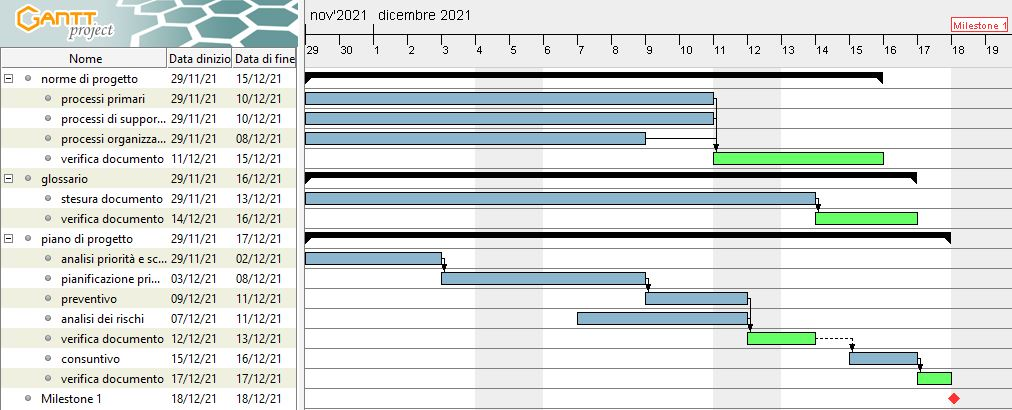
\includegraphics[width=1.0\textwidth]{Gantt1}
    \caption{Diagramma di Gantt della prima milestone} 
\end{figure}

\subsection{Secondo periodo}

\textit{Periodo: 20/12/2021 - 14/01/2022}

In questa fase diventa importante analizzare nel dettaglio il capitolato per riuscire a
cogliere tutti i requisiti necessari. Inoltre, per non avere dubbi e per non intraprendere
scelte sbagliate, sarà opportuno organizzare uno o più incontri con il proponente in modo da
condividere idee e dubbi sorti durante l'analisi che sarà sicuramente più approfondita di quella
effettuata durante la scelta del capitolato.
\par Da tutto ciò nascerà l'Analisi dei requisiti, documento importantissimo per il progetto poichè
conterrà tutti i casi d'uso, i requisiti obbligatori, quelli desiderabili e quelli opzionali.
\par In questa fase è opportuno stilare anche il Piano di Qualifica, necessario per individuare
i metodi per garantire la qualità di processo e di prodotto.

\begin{figure}[!ht]
    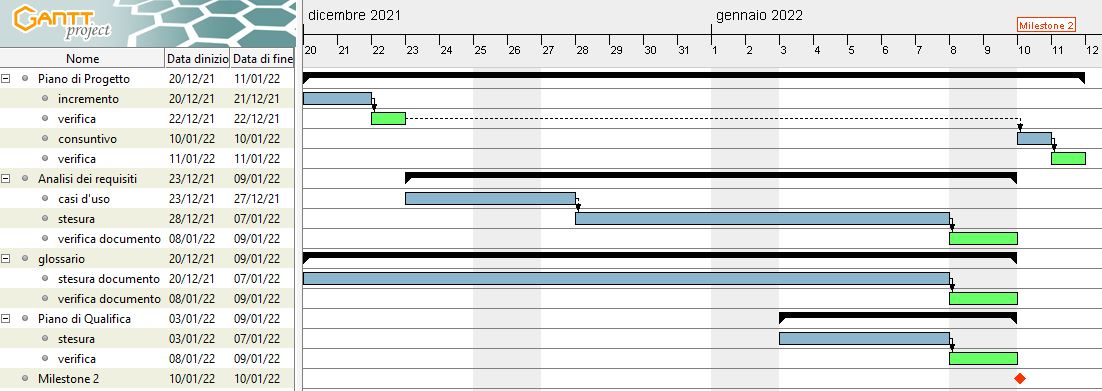
\includegraphics[width=1.0\textwidth]{Gantt2}
    \caption{Diagramma di Gantt della seconda milestone} 
\end{figure}

\subsection{Terzo periodo}

\textit{Periodo: 15/01/2022 - 24/02/2022}

Con l'Analisi dei requisiti scritta, diventa fondamentale studiare le tecnologie e gli strumenti necessari
per realizzare il prodotto. Questo permetterà di realizzare il PoC (Proof of Concept), una versione semplificata 
del prodotto finale che permetta di intuire se la direzione è quella giusta e che mostri al proponente se lo 
sviluppo è corretto.

\begin{figure}[!ht]
    %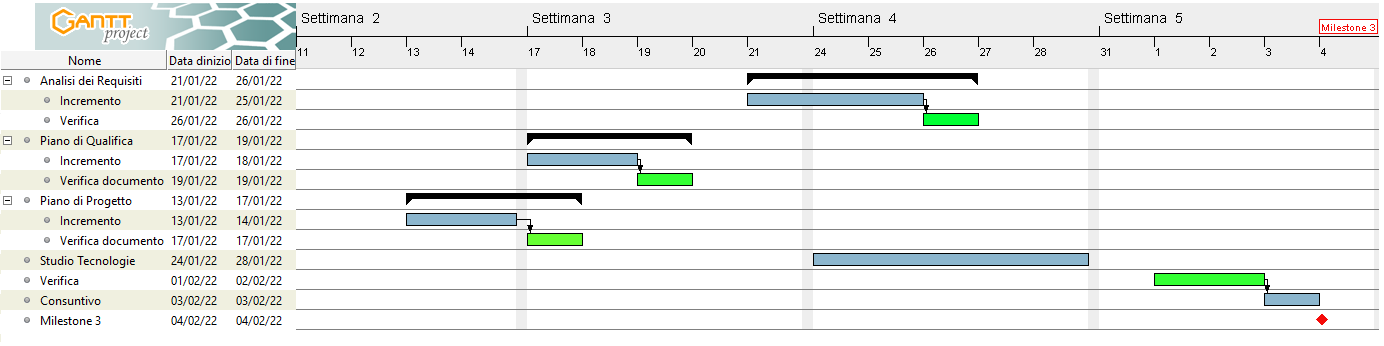
\includegraphics[width=1.0\textwidth]{Gantt3}
    \caption{Diagramma di Gantt della terza milestone} 
\end{figure}

\section{Verso la PB}

\textit{Periodo: 28/02/2022 - 31/03/2022}

\section{Verso la CA}

\textit{Periodo: 04/04/2022 - 05/05/2022}